We now describe the different standard computational blocks encountered in CNNs. 
We represent each block as a function $f$ which input is a matrix $\mathbf{x}$, and which output is a matrix
$\mathbf{y}$. The weights of the filter, when they exist, are denoted as the matrix $\mathbf{w}$.

  \begin{center}
  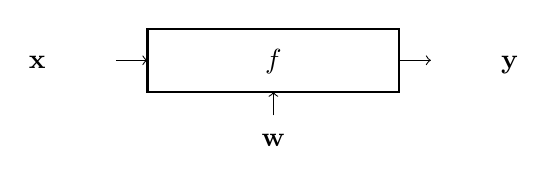
\begin{tikzpicture}
    \pgftext[base, x=   0cm, y= 0cm] {$f$}; 
    \pgftext[base, x=  -3cm, y= 0cm] {$\mathbf{x}$}; 
    \pgftext[base, x=   3cm, y= 0cm] {$\mathbf{y}$}; 
    \pgftext[base, x=   0cm, y=-1cm] {$\mathbf{w}$}; 
    \draw[black,thick] (-1.6cm,-0.3cm) rectangle (1.6cm,0.5cm); 
    \draw[->] ( -2cm, 0.1cm) -- (-1.6cm, 0.1cm);
    \draw[->] (1.6cm, 0.1cm) -- (   2cm, 0.1cm);
    \draw[->] (  0cm,-0.6cm) -- (   0cm,-0.3cm);
  \end{tikzpicture}
  \end{center}
  
For each block, we describe its formulation in a forward computation $\mathbf{y} = f(\mathbf{x},\mathbf{w})$.
We also provide the derivative of its output with respect to its input $\frac{dy}{dx}$. In order to be more explicit, we mention here the derivative 
of each output component with respect to each input component: $\frac{dy_{k_2}}{dx_{k_1}}$, where $k_1$ describes the dimension of the block input 
$\mathbf{x}$ and $k_2$ describes the dimension of the block output $\mathbf{y}$.  
These formulations can then be replaced in the equation %\ref{}
, allowing to compute the derivative of the CNN output $z$ with respect to each 


In the following section, $\delta$ is the Kronecker symbol: 
\begin{align}
  \delta_{proposition} &= 1 \hspace{0.2cm} \text{if} \hspace{0.2cm}  proposition \hspace{0.2cm} \text{is true}, \nonumber \\ 
                       &= 0 \hspace{0.2cm} \text{otherwise}. \nonumber
\end{align}